% Raphael Reitzig, 2012.
% MIT license

% Get an image by compiling to PDF and then
% > convert -density 600 tex_55948.pdf out.png
% > rm out-0.png
% > montage -geometry +3+2 -density 600 out-*.png out.png
% > mogrify -resize "750>x" out.png

\documentclass{article}
\usepackage[utf8]{inputenc}
\usepackage{xcolor,tikz,xifthen}
\usepackage[paperwidth=4cm,paperheight=3.25cm,margin=.5cm]{geometry}
\usetikzlibrary{positioning}

\tikzset{%
  active/.style={fill=yellow!30},
  unvisited/.style={opacity=.2},
  hidden/.style={opacity=0},
  lb/.style={color=green!70!black,scale=.7},
  ub/.style={color=red!70!black,scale=.7}
}

\begin{document}
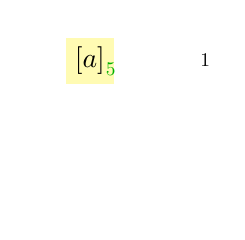
\begin{tikzpicture}[level 1/.style={sibling distance=10mm}]
  \node [active] (a) {$[a]$}
    child [hidden] { node (b) {$[b]$} }
    child [hidden] { node (c) {$[c]$} };

  \node[style=lb,below right=-3.5mm and -2mm of a] {$5$};
  \node[style=hidden,above right=-3.5mm and -2mm of a] {$5$};

  \node[style=hidden,below right=-3.5mm and -2mm of b] {$6$};
  \node[style=hidden,above right=-3.5mm and -2mm of b] {$7$};

  \node[style=hidden,below right=-3.5mm and -2mm of c] {$5$};
  \node[style=hidden,above right=-3.5mm and -2mm of c] {$5$};

  \node[right=1cm of a,scale=.7] {$1$};
\end{tikzpicture}
\clearpage

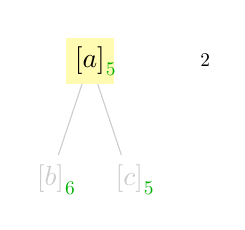
\begin{tikzpicture}[level 1/.style={sibling distance=10mm}]
  \node [active] (a) {$[a]$}
    child [unvisited] { node (b) {$[b]$} }
    child [unvisited] { node (c) {$[c]$} };

  \node[style=lb,below right=-3.5mm and -2mm of a] {$5$};
  \node[style=hidden,above right=-3.5mm and -2mm of a] {$5$};

  \node[style=lb,below right=-3.5mm and -2mm of b] {$6$};
  \node[style=hidden,above right=-3.5mm and -2mm of b] {$7$};

  \node[style=lb,below right=-3.5mm and -2mm of c] {$5$};
  \node[style=hidden,above right=-3.5mm and -2mm of c] {$5$};

  \node[right=1cm of a,scale=.7] {$2$};
\end{tikzpicture}
\clearpage

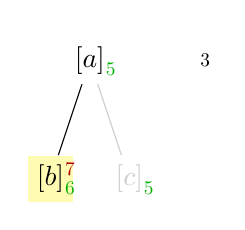
\begin{tikzpicture}[level 1/.style={sibling distance=10mm}]
  \node (a) {$[a]$}
    child { node [active] (b) {$[b]$} }
    child [unvisited] { node (c) {$[c]$} };

  \node[style=lb,below right=-3.5mm and -2mm of a] {$5$};
  \node[style=hidden,above right=-3.5mm and -2mm of a] {$5$};

  \node[style=lb,below right=-3.5mm and -2mm of b] {$6$};
  \node[style=ub,above right=-3.5mm and -2mm of b] {$7$};

  \node[style=lb,below right=-3.5mm and -2mm of c] {$5$};
  \node[style=hidden,above right=-3.5mm and -2mm of c] {$5$};

  \node[right=1cm of a,scale=.7] {$3$};
\end{tikzpicture}
\clearpage

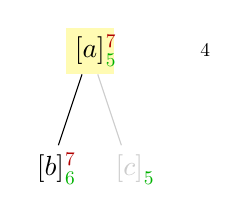
\begin{tikzpicture}[level 1/.style={sibling distance=10mm}]
  \node [active] (a) {$[a]$}
    child { node (b) {$[b]$} }
    child [unvisited] { node (c) {$[c]$} };

  \node[style=lb,below right=-3.5mm and -2mm of a] {$5$};
  \node[style=ub,above right=-3.5mm and -2mm of a] {$7$};

  \node[style=lb,below right=-3.5mm and -2mm of b] {$6$};
  \node[style=ub,above right=-3.5mm and -2mm of b] {$7$};

  \node[style=lb,below right=-3.5mm and -2mm of c] {$5$};
  \node[style=hidden,above right=-3.5mm and -2mm of c] {$5$};

  \node[right=1cm of a,scale=.7] {$4$};
\end{tikzpicture}
\clearpage

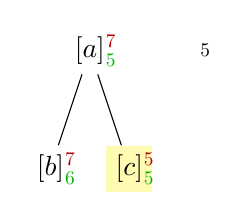
\begin{tikzpicture}[level 1/.style={sibling distance=10mm}]
  \node (a) {$[a]$}
    child { node (b) {$[b]$} }
    child { node [active] (c) {$[c]$} };

  \node[style=lb,below right=-3.5mm and -2mm of a] {$5$};
  \node[style=ub,above right=-3.5mm and -2mm of a] {$7$};

  \node[style=lb,below right=-3.5mm and -2mm of b] {$6$};
  \node[style=ub,above right=-3.5mm and -2mm of b] {$7$};

  \node[style=lb,below right=-3.5mm and -2mm of c] {$5$};
  \node[style=ub,above right=-3.5mm and -2mm of c] {$5$};

  \node[right=1cm of a,scale=.7] {$5$};
\end{tikzpicture}
\clearpage

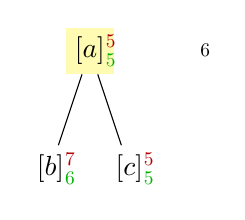
\begin{tikzpicture}[level 1/.style={sibling distance=10mm}]
  \node [active] (a) {$[a]$}
    child { node (b) {$[b]$} }
    child { node (c) {$[c]$} };

  \node[style=lb,below right=-3.5mm and -2mm of a] {$5$};
  \node[style=ub,above right=-3.5mm and -2mm of a] {$5$};

  \node[style=lb,below right=-3.5mm and -2mm of b] {$6$};
  \node[style=ub,above right=-3.5mm and -2mm of b] {$7$};

  \node[style=lb,below right=-3.5mm and -2mm of c] {$5$};
  \node[style=ub,above right=-3.5mm and -2mm of c] {$5$};

  \node[right=1cm of a,scale=.7] {$6$};
\end{tikzpicture}
\clearpage

\end{document}
